
\chapter{Introduction to Docsumo DataVerse 2023}
\section{Abstract}
ArXiv is a public service repository and open-source archive for scholarly articles in the fields of physics, mathematics, computer science, quantitative biology, quantitative finance, statistics, electrical engineering and systems science, and economics.

\section{Problem Description}
In this data challenge, Datasets that contains abstracts and categories columns that are collected from the arXiv portal are given to the participants. There are altogether 157 subject categories. For this competition, datasets having 23 classes are provided.

The task is to build a model to predict the category given paper abstract and title.

\section{Evaluation Metric}
The evaluation metric for this competition is Mean F1-Score. The F1 score, commonly used in information retrieval, measures accuracy using the statistics precision(\text{p}) and recall(\text{r}).

Precision is the ratio of true positives (\text{tp}) to all predicted positives (\text{tp} + \text{fp}). Recall is the ratio of true positives (\text{tp}) to all actual positives (\text{tp} + \text{fn}).

The F1 score is given by:

\[ \text{F1} = 2\frac{\text{p} \cdot \text{r}}{\text{p}+\text{r}}\ \ \mathrm{where}\ \ \text{p} = \frac{\text{tp}}{\text{tp}+\text{fp}},\ \ \text{r} = \frac{\text{tp}}{\text{tp}+\text{fn}} \]

The F1 metric weights recall and precision equally, and a good retrieval algorithm will maximize both precision and recall simultaneously. Thus, moderately good performance on both will be favored over extremely good performance on one and poor performance on the other.



\section{Dataset Overview}
Participants were given three files.
\begin{enumerate}
    \item \textbf{train.csv} : the training set
    \item \textbf{test.csv} : the test set
    \item \textbf{sample\_submission.csv} : a sample submission file in the correct format
\end{enumerate}

\subsection{Train Dataset Overview}
The train dataset contains total four columns as follow:
\begin{enumerate}
    \item \textbf{id} : Unique id of the article
    \item \textbf{title} : Title of the article
    \item \textbf{abstract} : Abstract of the article
    \item \textbf{category} :  Label of the article
\end{enumerate}

\begin{figure}[H]
    \centering
    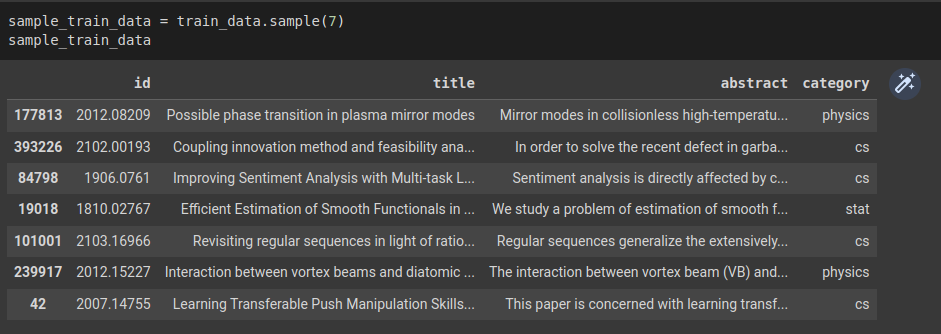
\includegraphics[scale = 0.5]{sample_train_data.png}
    \caption{Train Data Sample}
    \label{fig:Train Data Sample}
\end{figure}

Altogether, there are 8,61,236 entries in the training dataset. None of id, title and abstract column are null. However, 4 row for category column are null. The train dataset is of size 995.08 MB.

\begin{figure}[H]
    \centering
    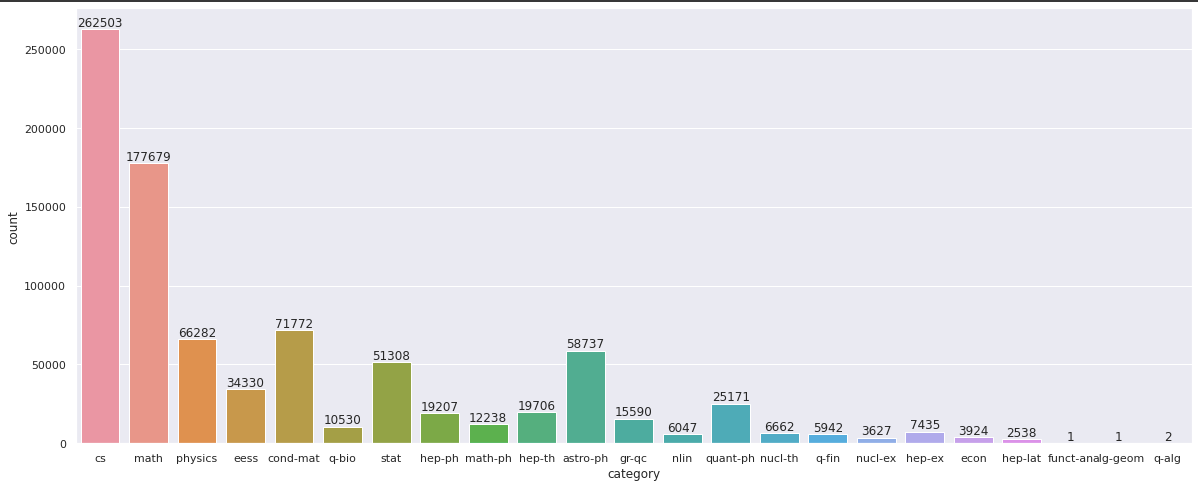
\includegraphics[scale = 0.4]{train_data_category.png}
    \caption{Train Data Category Countplot}
    \label{fig:Train Data Category Countplot}
\end{figure}

The name of the categories in the train data are cs, math, physics, eess, cond-mat, q-bio, stat, hep-ph, math-ph, hep-th, astro-ph, gr-qc, nlin, quant-ph, nucl-th, q-fin, nucl-ex, hep-ex, econ,
hep-lat, funct-an, alg-geom, and q-alg.

From the graph, we can observe that the count of some labels like cs, math, physics, cond-mat, astro-ph are greater than 50,000 while some labels have their count range from 2,000 to 30,000 and label "funct-an", "alg-geom" and "q-alg" have 2, 1 and 1 count respectively.

So, it is clear that the given training data is highly imbalanced and so we have to take the imbalanced into consideration. Otherwise, the model will be highly biased toward the majority class. Hence, we will have to use various sampling methods to balance the data and feed to the model for increasing the reliablility of the classifier model.

Some sample title and their category are shown below:
\begin{table}[H]
    \begin{center}
        \begin{tabular}{ |c|c|c| }
            \hline
            id         & title                                                               & category \\
            \hline
            2012.08209 & Possible phase transition in plasma mirror modes
                       & physics                                                                        \\

            \hline
            2102.00193 & Coupling innovation method and feasibility analysis of garbage
                       & cs                                                                             \\

            \hline
            1810.02767 & Efficient Estimation of Smooth Functionals in Gaussian Shift Models & stat     \\
            \hline
        \end{tabular}
    \end{center}
    \caption{Train Data Title Category Sample}
    \label{table:Train Data Title Category Sample}
\end{table}

\subsection{Test Dataset Overview}
The test dataset contains total of four columns : id, title,abstract and category. The size of test dataset is of 52.13 MB. There are 43,785 entries in the test dataset. 

\begin{figure}[H]
    \centering
    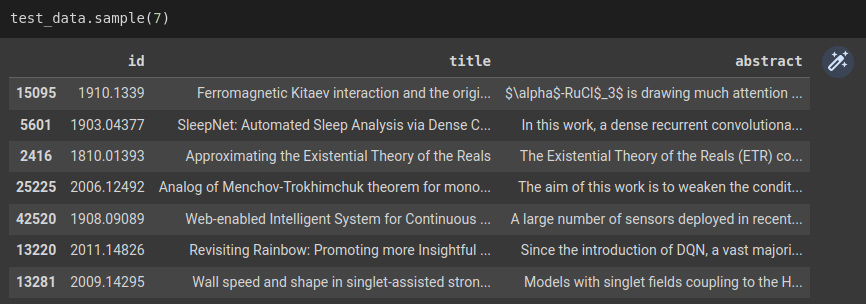
\includegraphics[scale = 0.55]{test_data_sample.png}
    \caption{Test Data Sample}
    \label{fig:Test Data Sample}
\end{figure}

\subsection{Submission Format}
For every author in the dataset, submission files should contain two columns: ID and Category. The file should contain a header and have the following format in csv file:

The file should contain a header and have the following format:

\begin{figure}[H]
    \centering
    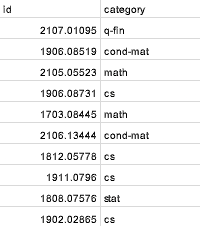
\includegraphics[scale = 1]{submission.png}
    \caption{Submission File Format}
    \label{fig:Submission File Format}
\end{figure}